\subsection{Introduction}
The goal of this first part is to implement a minimal working simulation of a QAM communication.
In order to achieve that, the up- and downsampling blocks, the RRC filtering blocks and the baseband equivalent model of the channel, as represented in figure~\ref{fig:chain} must be implemented.
\begin{figure}[htbp]
\centering

\caption{Block diagram of the communication system [source: Assignment introduction].\label{fig:chain}}
\end{figure}
The modulator and demodulator are supplied with the assignment statement.

\subsection{Halfroot Nyquist filtering}
After its modulation, the message is upsampled and filtered with a root raised cosine filter to limit its bandwidth occupation.
The effect on the PSD of the signal is shown in figure~\ref{fig:LPF}.
\begin{figure}[htbp]
\centering
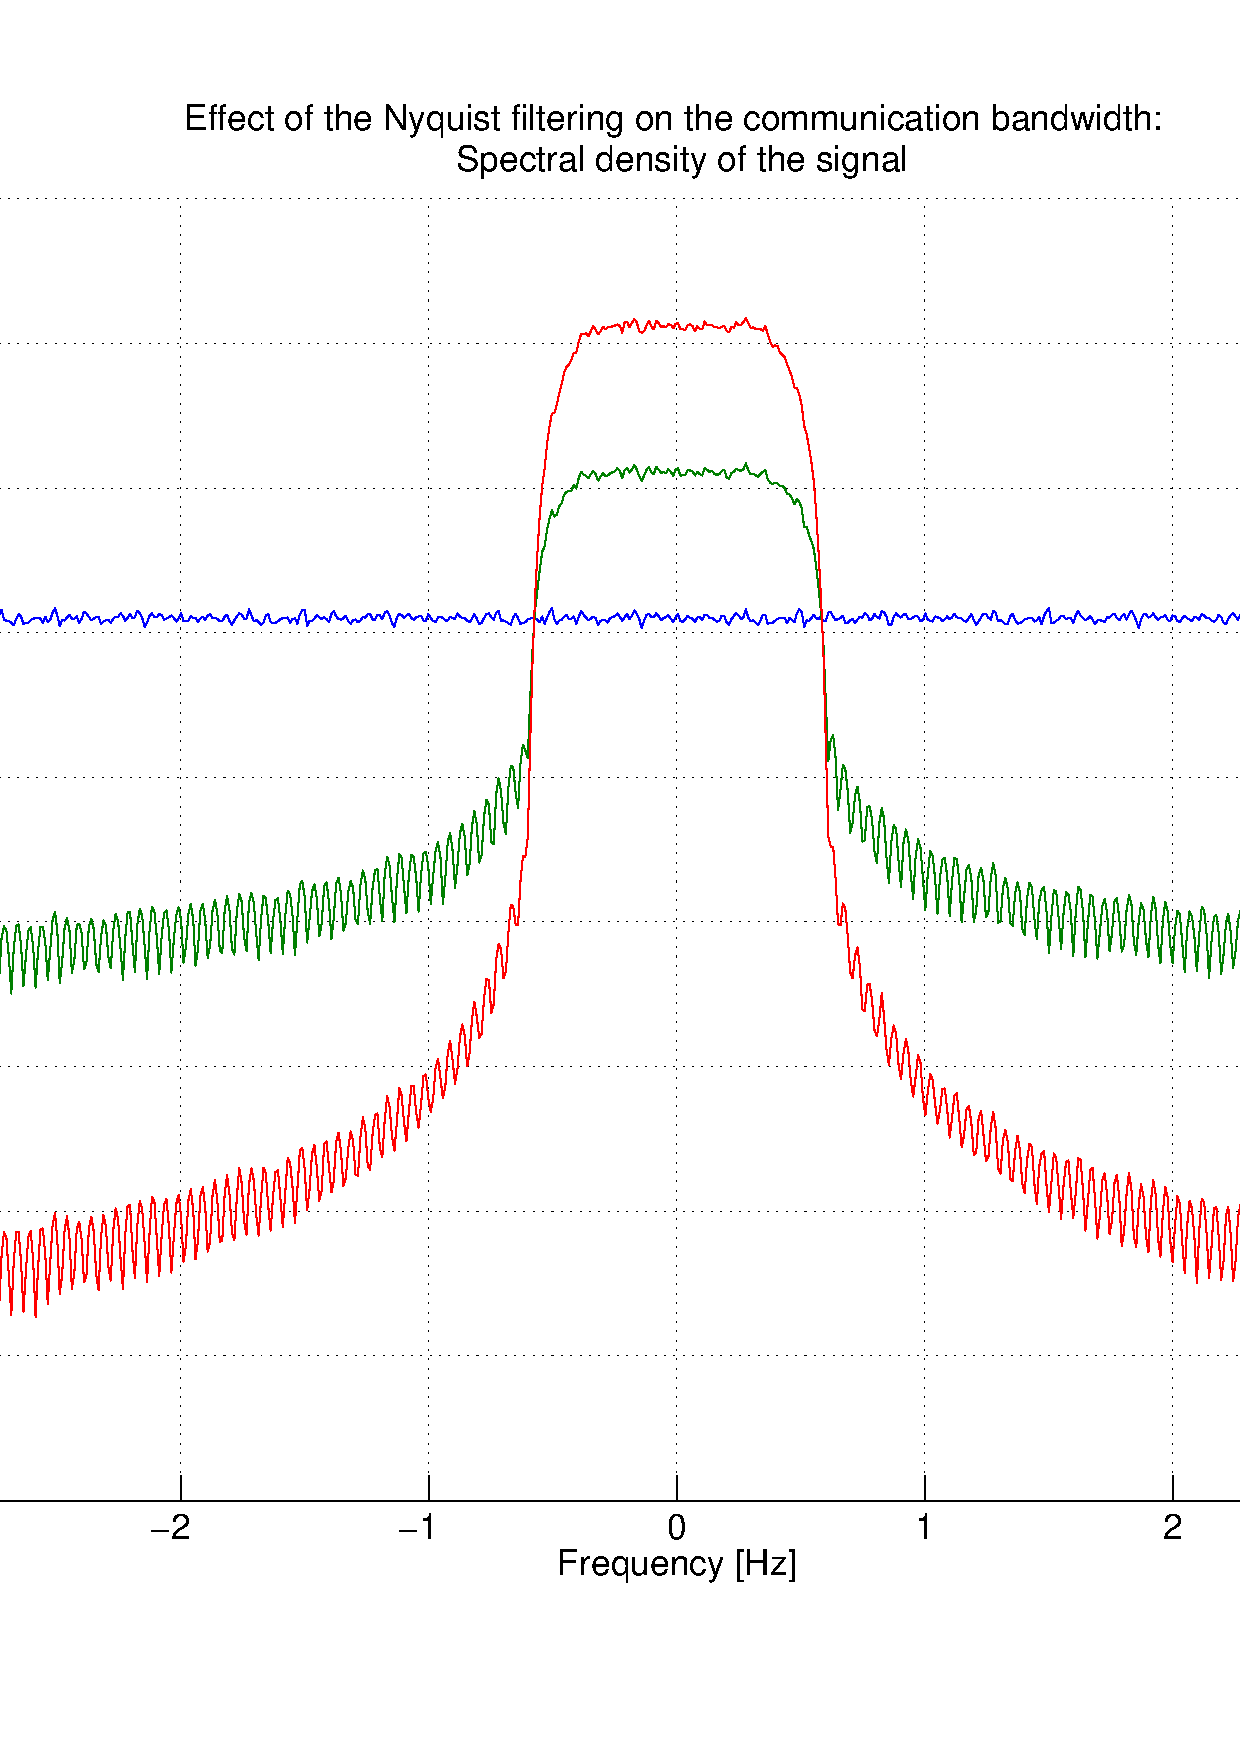
\includegraphics[width=\textwidth]{commBW.pdf}
\caption{Nyquist filtering limits the communication bandwidth.\label{fig:LPF}}
\end{figure}

I order to maximize the SNR at the output, the low pass filtering is split between the transmitter and the receiver.
The halfroot nyquist filter $g(t)$ is such that the resulting operation $h(t) = g(t)*g(t)$ forms a nyquist filter which does not introduce inter symbol interference, as shown in figure~\ref{fig:noISI}
\begin{figure}
\centering
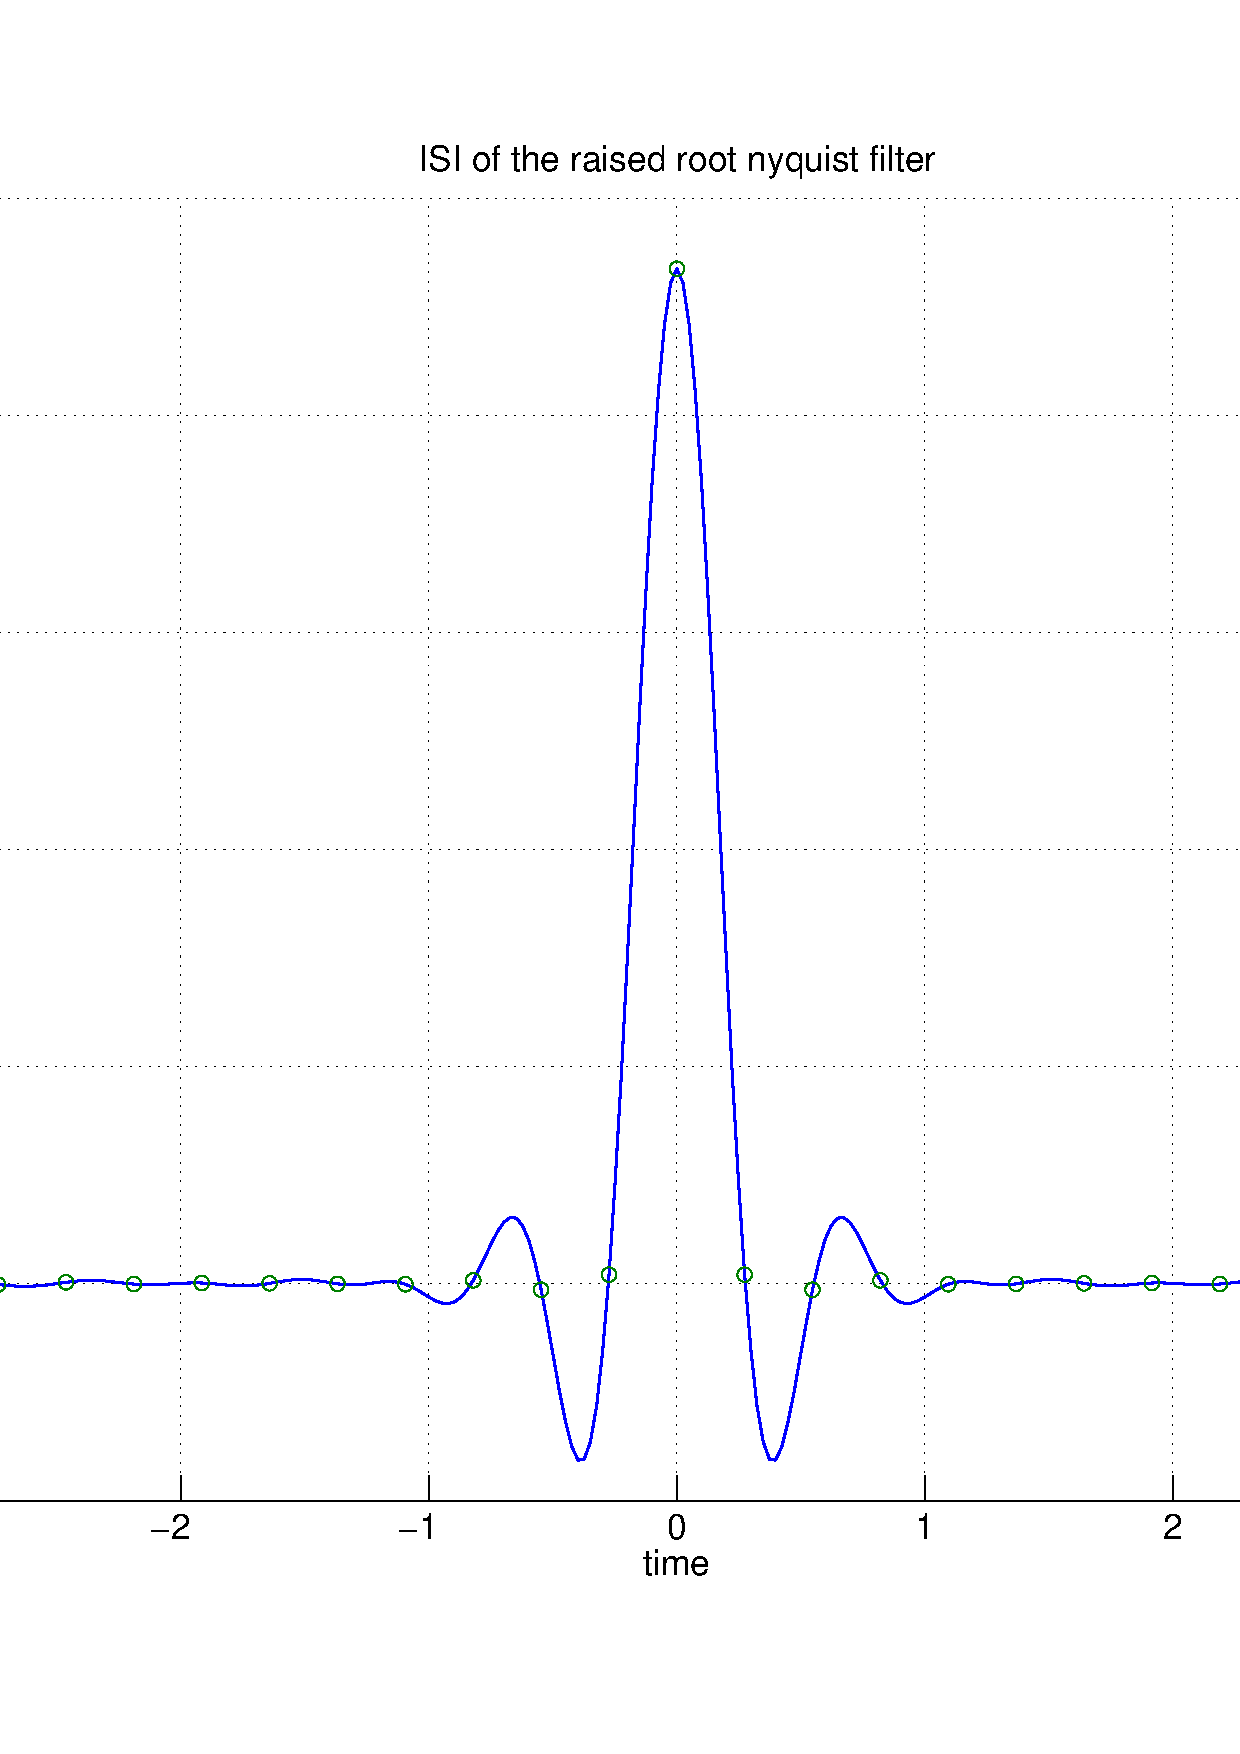
\includegraphics[width = \textwidth]{isi.pdf}
\caption{Cancellation of the inter symbol interference of a raised cosine filter.\label{fig:noISI}}
\end{figure}

\subsection{Impact of the noisy channel}
Theory shows that a channel affected by AWGN can be modelled in the baseband by AWGN of corresponding power.
This allows to easily simulate the BER of the noisy channel.
The results of the simulations are summarized by the BER curves of figure~\ref{fig:BER}
\begin{figure}[htbp]
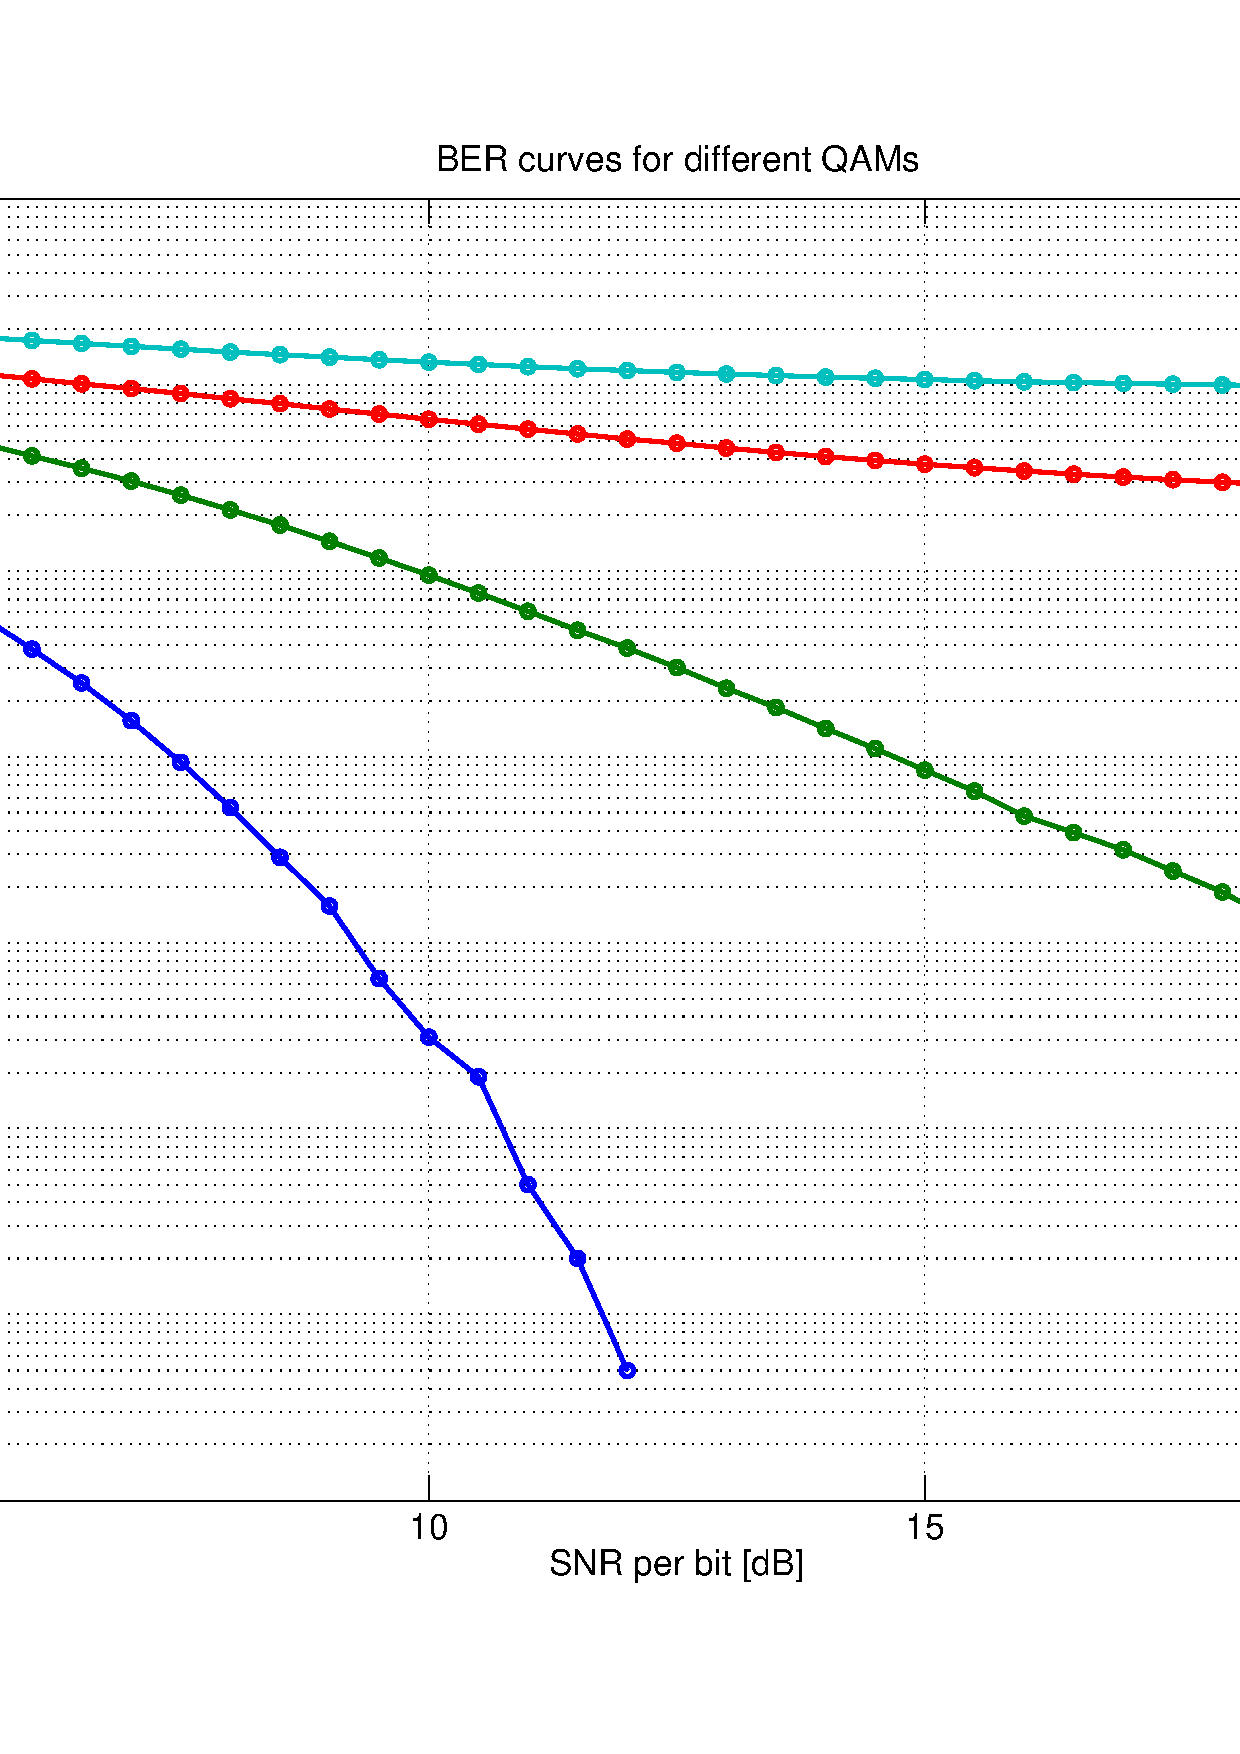
\includegraphics[width=\textwidth]{BERs.pdf}
\caption{BER in function of $\frac{E_b}{N_0}$ for different QAM modulations.\label{fig:BER}}
\end{figure}

\subsection{Questions}
\subsubsection{Simulation}
\paragraph{It is proposed to use the baseband equivalent model of the AWGN channel. Would it be
possible to live with a bandpass implementation of the system?}
\paragraph{How do you choose the sample rate in Matlab?}
\paragraph{How do you make sure you simulate the desired $\frac{E_b}{N_0}$ ratio?}
\paragraph{How do you choose the number of transmitted data packets and their length?}

